
\documentclass[conference]{IEEEtran}


%\usepackage{multirow}
%\usepackage{rotating}
%\usepackage{array}
\usepackage{color}
%\usepackage{verbatim}
%\usepackage{subfigure}
%\usepackage{bigstrut}
%\usepackage{amsmath}
%\usepackage{color}
%\usepackage{comment}



\usepackage{cite}
%\usepackage{graphicx}
\usepackage{listings}
%\usepackage{pxfonts}
%\usepackage{times}
%\usepackage{xspace}
%\usepackage{booktabs}
%\usepackage{fancybox}
%\usepackage{color}
%\usepackage{multirow}
%\usepackage{array}
%\usepackage{tabularx}
%\usepackage{url}
%\urlstyle{same}
%\usepackage{xcolor}
%\usepackage{pgfplots}
%\usepackage{tikz}
%\usepackage{caption}
%\usetikzlibrary{shapes,arrows, positioning}
%\usetikzlibrary{patterns}
%\usepackage[numbers]{natbib} % Used to fix formatting issue.
%\usepackage{soul} % Needed for wrapping of highlighted text
%\usepackage{balance} % Used to balance out the columns



\usepackage{cite}
\usepackage{color}
%\usepackage{courier}
\usepackage{listings}
%\usepackage{url}
%\usepackage{balance} % Add this back in. Probably needed during camera ready.
%\usepackage{listings} % Not sure this does anything here
\usepackage{tikz} % Need for all tikz material
%\usetikzlibrary{shapes,arrows, positioning} %  Need for all tikz material
%\usepackage{balance}

\usepackage{times} % Used for formatting formatting url footnotes
%\urlstyle{same} % Used for formatting formatting url footnotes
%\usepackage{caption} % Used for formatting formatting url footnotes
%\usepackage{graphicx}
%\usepackage{subcaption}


\newcommand{\mehdi}[1]{\textcolor{red}{{\it [Mehdi says: #1]}}}
\newcommand{\dan}[1]{\textcolor{blue}{{\it [Dan says: #1]}}}


\lstset{ %
language=java,                % choose the language of the code
%xleftmargin=100pt,xrightmargin=100pt
basicstyle=\footnotesize,       % the size of the fonts that are used for the code
%numbers=left,                   % where to put the line-numbers
numberstyle=\footnotesize,      % the size of the fonts that are used for the line-numbers
stepnumber=1,                   % the step between two line-numbers. If it is 1 each line will be numbered
numbersep=3pt,                  % how far the line-numbers are from the code
backgroundcolor=\color{white},  % choose the background color. You must add \usepackage{color}
showspaces=false,               % show spaces adding particular underscores
showstringspaces=false,         % underline spaces within strings
showtabs=false,                 % show tabs within strings adding particular underscores
frame=none,           % adds a frame around the code
tabsize=2,          % sets default tabsize to 2 spaces
captionpos=t,           % sets the caption-position to bottom
%captionpos=b,           % sets the caption-position to bottom
breaklines=true,        % sets automatic line breaking
breakatwhitespace=false,    % sets if automatic breaks should only happen at whitespace
escapeinside={\%*}{*)}          % if you want to add a comment within your code
}

\setlength{\abovecaptionskip}{6pt plus 3pt minus 2pt} % Space over captions
%\setlength{\belowcaptionskip}{6pt plus 3pt minus 2pt} % Space under captions



\lstdefinestyle{ConcolicOutput}{
   % language={SQL},basicstyle=\ttfamily,
    moredelim=**[is][\btHL]{`}{`},
   % moredelim=**[is][{\btHL[fill=green!30,draw=red,dashed,thin]}]{@}{@},
}



\begin{document}
%
% paper title
% can use linebreaks \\ within to get better formatting as desired
\title{Architectural Clones: Toward Tactical Code Reuse}

\author{\IEEEauthorblockN{Mehdi Mirakhorli and Daniel E. Krutz}
\IEEEauthorblockA{
Software Engineering Department\\
Rochester Institute of Technology,
Rochester, NY, USA\\
\{mxmvse,dxkvse\}@rit.edu}
}




% use for special paper notices
%\IEEEspecialpapernotice{(Invited Paper)}




% make the title area
\maketitle


\begin{abstract}
%\boldmath

Architectural tactics are building blocks of software architecture. They describe solutions for addressing specific quality concerns, and are prevalent across many software systems. Once a decision is made to utilize a tactic, the developer must generate a concrete plan for implementing the tactic in the code. Unfortunately, this a non-trivial task for many inexperienced developers. Developers often use code search engines, crowd-sourcing websites, or discussion forums to find sample code snippets. A robust tactic recommender system can replace this manual internet based search process and assist developers to reuse successful architectural knowledge, as well as implementation of tactics and patterns  from a wide range of open source systems. In this paper we study several implementations of architectural choices in the open source community and identify the foundation of building a practical tactic recommender system. As a result of this study we introduce the concept of~\emph{tactical-clones} and use that as a basic element to develop our recommender system. While this NIER paper does not present the details of our recommender engine, instead it proposes the basis of our architecture recommender system.

\end{abstract}
% IEEEtran.cls defaults to using nonbold math in the Abstract.
% This preserves the distinction between vectors and scalars. However,
% if the conference you are submitting to favors bold math in the abstract,
% then you can use LaTeX's standard command \boldmath at the very start
% of the abstract to achieve this. Many IEEE journals/conferences frown on
% math in the abstract anyway.

% no keywords




% For peer review papers, you can put extra information on the cover
% page as needed:
% \ifCLASSOPTIONpeerreview
% \begin{center} \bfseries EDICS Category: 3-BBND \end{center}
% \fi
%
% For peerreview papers, this IEEEtran command inserts a page break and
% creates the second title. It will be ignored for other modes.
\IEEEpeerreviewmaketitle



\section{Introduction}
The success of any complex software-intensive system is dependent on how it addresses quality attribute concerns of the stakeholders. Some include security, usability, availability, and interoperability. Designing a system to satisfy these concerns involves devising and comparing alternate solutions, understanding their trade-offs, and ultimately making a series of design choices. These architectural decisions typically begin with design primitives such as architectural tactics and patterns.

Tactics are the building blocks of architectural design \cite{bass:arch12}, reflecting the fundamental choices that an architect makes to address a quality attribute concern. Because they are building blocks, tactics are composed together to form patterns. Architectural tactics come in many different shapes and sizes and describe solutions for a wide range of quality concerns. They are particularly prevalent across high-performance and/or fault tolerant software systems. Reliability tactics such as~\emph{redundancy with voting},~\emph{heartbeat}, and~\emph{check pointing} provide solutions for fault mitigation, detection, and recovery; while performance tactics such as~\emph{resource pooling} and~\emph{scheduling} help optimize response time and latency.

The importance of implementing architectural tactics rigorously and robustly was highlighted by a small study we conducted as a precursor to this work. We investigated tactic implementations in Hadoop  and OFBiz and evaluated their degree of stability during the maintenance process. For each of these projects we retrieved a list of bug fixes from the change logs (Nov. 2008 - Nov. 2011 for Hadoop, and Jan. 2009 - Nov. 2011 for OFBiz). Our analysis showed that tactics-related classes incurred 2.8 times as many bugs in Hadoop, and 2.0 times as many bugs in OFBiz as non-tactics related classes. In another preliminary work, we studied the implementation of security tactics in Chromium Browser and we observed that 10\% of tactic implementations resulted in reported  vulnerabilities. These observations suggest that tactic implementations, if not developed correctly, are likely to contribute towards the well-documented problem of architectural degradation \cite{Erosion}. Less experienced developers sometimes find this challenging, primarily because of the variability points that exist in a tactic, and the numerous design decisions that need to be made in order to implement a tactic in a robust and effective way. We found many examples of such questions on coding forums.

A robust tactic recommender system that shares sample code snippets from successful implementation of tactics in open source community can provide valuable support for the developers. Unfortunately, obtaining a practical tactic recommender system is not an simple task. This paper discusses the foundation of such a recommender system. Although there have been some initial development of source code recommender systems~\cite{DBLP:conf/icse/McMillanHPCM12,6340250}, the primary focus of such works are on generic codes and not tactical codes. Therefore the challenges of obtaining and recommending architecturally significant code is still unexplored.
Prior to proposing more specific guidelines for developing an architecture recommender system, we conducted an extensive study of architectural decisions in performance centric and dependable complex system. This study provided the foundation and motivation for the introduction of the concept of ``Tactical Clones''. We investigate this notion in several open source systems and use them as key elements in developing our recommender system.
\vspace{-10pt}
\section{Tactic's Implementation: Seen and Unseen}
Our study involved review the source code of over 50 complex, performance centric open source systems including projects such as Google Chromium, Apache Hadoop, and Camel projects. For each of the studied projects we identified architecturally significant requirements, architectural tactics used to address them and source files used to implement tactics.
As a result of this study we observed five issues that significantly influence development of any practical architecture recommender system. Each of these is discussed below:


\noindent \textbf{$\bullet$ No Single Solution.}
There is no single way to address a quality requirements and also no single way to implement an architectural tactic. From one system to another system a tactic can be implemented entirely differently, this divergence is due to the differences in the context and constraints of each projects.
For example, we reviewed the implementation of \emph{heartbeat} tactic for reliability concerns in 25 different software systems. We observed the heartbeat tactic being implemented using (i) direct communication between the emitter and receiver roles found in~\emph{(Chat3 and Smartfrog systems)}, (ii) the observer pattern in which the receiver is registered as a listener to the emitter found in the \emph{Amalgam system}, (iii) the decorator pattern in which the heartbeat functionality was added as a wrapper to a core service found in~\emph{(Rossume} and~\emph{jworkosgi systems)}, and finally (iv) numerous proprietary implementations which did not follow any documented design notion.
Therefore a recommender system can not primarily rely on structural dependencies as a means of learning the best tactic implementation.

\noindent \textbf{$\bullet$ Structure Is Not a Key, But Impacts Quality.}
Unlike design patterns, which tend to be described in terms of classes and their associations , tactics are described in terms of roles and interactions \cite{bass:arch12}.  This means a tactic is not dependent upon a specific {\em structural} format. While a single tactic might be implemented using a variety of design notions or proprietary designs, the structural properties of tactical files can have significant on the quality of the tactic. Flaws such as cyclic dependencies, improper inheritance, unstable interfaces, and modularity violations are strongly correlated to increased bug rates and increased costs of maintaining the software. For example we found several security bug reports on Stack Overflow website where developers misuses \emph{inheritance} relationship in implementation of \emph{sandbox} tactic. In those cases a process outside sandbox had inheritance relationship with a process inside sandbox resulting in a breach into secure zones of the project.
A recommender solution should take into account the internal quality of recommended code to avoid suggesting codes with design and structural flaws.

\noindent \textbf{$\bullet$ Tactical Clones: Right Level of Granularity.}
While the implementation of tactics are different from one system to another system, the intrinsic characteristics of tactics are maintained across different projects. We call these as \emph{architectural or tactical clones}. Based on our observation, tactical clones are the right level of granularity for recommending tactic implementations.
In our code review process, we found that even for a simple tactic like heartbeat the implementation would result in a large number of interrelated files, each playing different roles such as heartbeat emitter, heartbeat receiver, configuration files to set heartbeat intervals and other parameters, supporting classes and interfaces to implement each  tactical roles. More complex tactics, specially the cross-cutting ones can easily impact hundreds of source files. Therefore recommending code snippets for those tactics would create a large search space for the developers with lesser degree of reusability. The lack of structure, and a concrete micro-level design which can be recovered across multiple projects indicates that method level clones are the right level of granularity.  In the next section of this paper we provide examples of such tactical clones.

\noindent \textbf{$\bullet$ Tactics Are Misused, Degraded or Implemented Incorrectly.} Open source repositories contain several cases where architectural tactics have been adopted by the developers without fully understanding the driving forces and variability points \cite{FSE2012} associated with each tactic and consequences of implementing the tactic. The Heartbleed issue is a good example of such misuse. Heartbeat functionality in OpenSSL is an optional feature, while many developers could have easily disabled it in configuration files they fully ignored that. Furthermore, the implementation of heartbeat functionality did not followed solid software engineering practices.

In our analysis of bug reports in tactical fragments of the Hadoop project, we found that if a tactical file had a bug, then 89\% of these issues were due to issues such as unhandled exceptions, type mismatches, or missing values in a configuration file. 
11\% of reports where due to wrong implementation. These bugs involved misconceptions in the use of the tactic, so that the tactic failed to adequately accomplish its architectural task.  These kinds of bugs caused the system to crash under certain circumstances. For example, in one case a replication decision with a complex synchronization mechanism was misunderstood for different types of replica failure. Another example was a scheduling tactic which resulted in deadlock problem. This investigation shows that systems are exposed to new risks during implementation of the tactical decisions. A good tactic recommendation needs to take into account tactical code qualities, the context in which the tactics are adopted and the historical bug fixes and refactoring activities on candidate clone for recommendation. Our recommender system uses a set of static analysis tool to rank recommended tactical code clones based on their quality.

\noindent \textbf{$\bullet$ Object Oriented Metrics Are Not Indicator of Tactical Code Quality.}
Our initial analysis of Chidamber and Kemerer's OO metrics~\cite{491650} and tactical code snippets in Apache Hadoop and OfBiz systems indicates that tactical code snippets tend to relatively a have higher code complexity compared to non-tactical code snippets. For example implementing thread pooling requires devising solutions for thread safe problem which will results in a more complex implementation. Therefore OO metrics such as \emph{WMC (Weighted Methods per Class)} or~\emph{CBO (Coupling Between Object classes)} can not solely be a good indicator of an improved tactical code snippet. A good tactic recommender system must take into account novel code metrics to filter potentially complex code samples which are difficult to comprehend and modify.

\section{Architectural Clones: A Step Toward Tactical Code Reuse}
In order to illustrate the concepts of architectural or tactical clones we conducted an explorative study and established a representative sample of such design clones. To do so we developed a semi-automated process for retrieving candidate instances of tactic-related classes then detected code clones across these tactical files. The process involved the following steps (1) building a software repository, (2) extracting instances of architectural tactics, (3) extracting code clones across projects,  and finally (4) manually inspecting the results to investigate our hypothesis that tactical clones are a practical granularity for architectural reuse.

\noindent
\begin{table*}[ht]
\vspace{-2pt}
\caption{An Example HeartBeat Tactical Clone~\label{table:heartbeedexample}}
\centering
\begin{tabular}{c | c}
\bfseries HeartBeat Example \#1  & \bfseries HeartBeat Example \#2  \\ \hline \hline
\begin{lstlisting}
boolean shouldBeRunning=true;
int smallInterval=10;
long lastHeartbeat=0;
int heartbeatInterval=10;
while (shouldBeRunning){
  Thread.sleep(smallInterval);
  if(System.currentTimeMillis()-lastHeartbeat>
    heartbeatInterval){
    sendHeartbeat();
    lastHeartbeat= System.currentTimeMillis();
  }
}
\end{lstlisting}
&
\begin{lstlisting}
long lastRunTime=0;	
long timeSpan=System.currentTimeMillis();
long timeSinceLastRun=
  System.currentTimeMillis()-lastRunTime;
  if(timeSinceLastRun>10) {
    sendHeartbeat();
	lastRunTime = System.currentTimeMillis();
}
\end{lstlisting}

\end{tabular}
\vspace{-2pt}
\end{table*}
\vspace{-8pt}

\subsection{Building a software repository}
We preselected 37 open source projects with a high number of architectural tactics. These tactic rich projects were identified through a previous study \cite{FSE2014}.


\subsection{Extracting architectural tactics}

To identify architectural tactics, we utilized a previously developed tactic detection algorithm and tool \cite{ICSE2012, FSE2014}. This Tactic Detector's classifiers have been trained to detect architectural tactics such as \textit{audit trail}, \textit{asynchronous method invocation}, \textit{authentication}, \textit{checkpointing and roll back}, \textit{heartbeat}, \textit{role-based access control (RBAC)}, \textit{resource pooling}, \textit{scheduling}, \textit{ping echo}, \textit{hash-based method authentication}, \textit{kerberos} and \textit{secure session management}.
Due to space constraints we provide only an informal description of our tactic detection approach; however a more complete description of the approach, including its related formulas, is provided in other publications \cite{Dissertation, ICSE2012}.  The tactic detection technique uses a set of classification techniques. These classifiers are trained using code snippets representing different architectural tactics, collected from hundreds of high-performance, open-source projects \cite{FSE2012,ICSE2012,Dissertation}.  During the training phase, the classifier learns the terms (method and variable names as well as development APIs) that developers typically use to implement each  tactic and assigns each potential indicator term a weight with respect to each type of  tactic. The weight estimates how strongly an indicator term signals an architectural tactic. For instance, the term \emph{priority} is found more commonly in code related to the \emph{scheduling} tactic than in other kinds of code, and therefore the classifier assigns it a higher weighting with respect to scheduling. During the classification phase, the indicator terms are used to evaluate the likelihood that a given file implements an architectural tactic.

The accuracy of the Tactic Detector has been evaluated in several studies \cite{ICSE2012,FSE2014,Dissertation}. In a series of  experiments it was able to correctly reject approximately 77-100\% of non-tactical code classes (depending on tactic types); recall 100\% of the tactics-related classes with precision of 65\% to 100\% for most tactics tactics.  The recall for the authentication, audit trail and asynchronous method invocation was 70\% .

While this approach does not return entirely precise results, it has the a tuning parameter which enables us to only include the tactical files with higher prediction confidence in our analysis, which this will significantly reduce the search space and assist with the task of retrieving candidate tactical clones.


%The final projects are listed in Table \ref{tab:ChosenProjects}. For each project we report its name, the number of classes in the system, the number of tactic types covered (maximum 13), number of candidate design patterns detected (maximum 20), and the final count of pattern/tactic overlaps as predicted by our automated tools.  As depicted in this table, most of the included projects provided coverage of 5 or more tactic types; however in order to ensure coverage of all the studied tactics, we included a couple of additional projects simply because they included the targeted tactic type, even though their overall tactic coverage was low.

%%%%%%%%%%%%%%%%%%%%%%%%%%%%%%


\subsection{Detecting Tactical Clones}
In order to detect architectural clones we used code clone detection techniques to identify reused tactical methods across different projects.
We define the four types of tactical code clones using the definitions from Roy et al.~\cite{Roy:2008:NAD:1437898.1438600} for code clones.
Type-1 tactical clones are the simplest, representing identical tactical code except for variations in whitespace, comments, and layout to the type-4 clones, which are the most complex. Type-4 tactical clones, are tactical code segments that perform the same computation, but have been implemented using different syntactic variants. Our initial investigation indicates that type-4 or semantically equivalent tactical clones can be detected using complex code similarity techniques such as concolic and symbolic analysis \cite{wcre2013}

%with type-1 tactical clones being the simplest and easiest to detect all the way to type-4 tactical clones which are the most complicated and difficult to discover.


% . Type-1 clones are the simplest and easiest to detect

% Type-1 clones are the simplest, representing identical tactical code except for variations in whitespace, comments, and layout to the type-4 clones, which are the most complex. Type-4 tactical clones, the most difficult to detect, are tactical code segments that perform the same computation, but have been implemented using different syntactic variants. Concolic analysis ~\cite{Sen:2005:CCU:1081706.1081750} can be used to detect type-4 tactical clones~\cite{wcre2013}.

% Type-2 clones have variations in identifiers, types, whitespace, literals, layout, and comments, but are otherwise syntactically identical. Type-3 clones are tactical fragments which are copied and have modifications such as added or removed statements, variations in literals, identifiers, whitespace, layout and comments.

% Traditionally it has been used for software testing~\cite{Sen:2005:CCU:1081706.1081750}, code clone detection~\cite{wcre2013}, and vulnerability recognition~\cite{Chen:2014:CIB:2554850.2554875}.






Concolic analysis combines concrete and symbolic values to traverse all possible paths (up to a given length) of an application. Since concolic analysis is not affected by syntax or comments, identically traversed paths are indications of duplicate functionality, and therefore functionally equivalent code. These traversed paths are expressed in the form of~\emph{concolic output} which represents the execution path tree and displays the utilized path conditions and representative input variables. In order to detect tactical-clones we used a concolic analysis based clone detection technique \cite{wcre2013,Dan123} on two type-4 clone examples examples of heartbeat are shown in Table~\ref{table:heartbeedexample}.
\begin{figure*}[!t]
\vspace{-1pt}
\centering
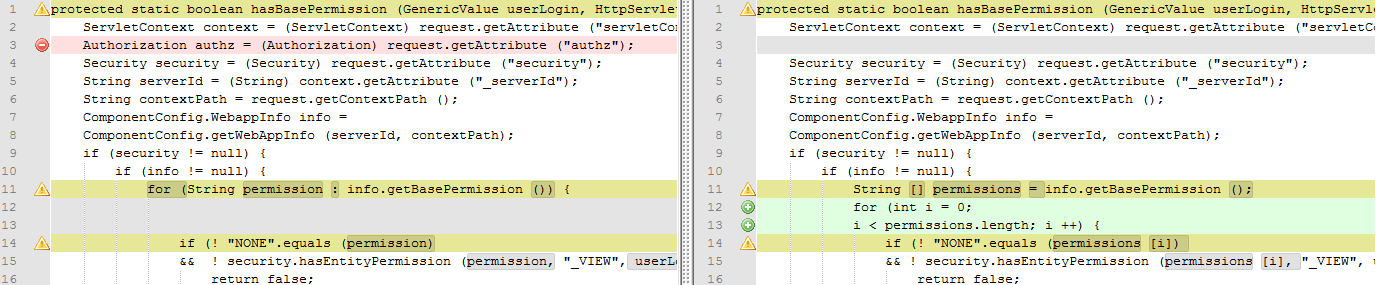
\includegraphics[width=0.9\linewidth]{./img/Permission}
\vspace{-6pt}
\caption{Tactical Clones Detected in Two different Projects}
\label{fig:Permission}
\vspace{-1pt}
\end{figure*}




We then ran concolic analysis on these two code segments which produced the matching concolic output shown in Table~\ref{fig:exampleoutput} which indicated that original code snippets are tactical clone type-4. In this example, variable type integers are represented by a generic tag ``SYMINT.'' Though not present in this example, other variable types are represented in a similar fashion in concolic output. Actual variable names do not appear anywhere in the output and are irrelevant to this clone detection process. We anticipate that open source repositories have a large number of tactical clone type-4 which can be used as items for a recommender system.


In an extensive experiment we ran a leading clone detection tool Nicad~\cite{Roy:2008:NAD:1437898.1438600}, over the tactical code snippets from 37 projects. We chose Nicad for our larger analysis since it is a more mature and refined tool than our experimental technique based upon concolic analysis. However, we believe that concolic analysis represents a more promising technique for tactical clone detection in our future work.




Table~\ref{tab:ChosenProjects} shows tactics used in our study, as well as the number of tactical clones across projects (Note: We do not report tactical clones within the same project). Last column of this table illustrates total number of tactical files used in this study. The tactical clones were detected at method level, although we could have detected them as sub-method level we realized that method level tactical clones are easier to comprehend and therefore easier to reuse for the developers. 


As a result of our explorative study we found several examples of identical tactical code snippets (type1,2 and 3) and several examples of conceptually equivalent tactical code snippets (type 4). Figure \ref{fig:Permission} shows the source code for RBAC tactic across two different projects. In this example two developers in different system have potentially developed the same code snippets to implement the tactic. This observation and several similar detected clones also emphasizes the fact that tactical clones are a more common granularity for code adoption and reuse.



\noindent
\begin{table}[hb] %h for here, t for top, b for bottom
\vspace{-16pt}
\caption{Diff of HeartBeat Concolic Output}
~\label{table:concolicoutputcomparision}
\centering
\begin{tabular}{ p{3.8cm} | p{3.8cm} }
\multicolumn{1}{c}{\textbf{Concolic Segment \#1}} & \multicolumn{1}{c}{\textbf{Concolic Segment \#2}} \\ \hline \hline
\begin{lstlisting}[style=ConcolicOutput]
### PCs: 1 1 0
a_1_SYMINT,
a_1_SYMINT,d1_2_SYMREAL,
a_1_SYMINT,d1_2_SYMREAL,s1_3_SYMSTRING,
\end{lstlisting}
&
\begin{lstlisting}[style=ConcolicOutput]
### PCs: 1 1 0
a_1_SYMINT,
a_1_SYMINT,d1_2_SYMREAL,
a_1_SYMINT,d1_2_SYMREAL,s1_3_SYMSTRING,
\end{lstlisting}

\end{tabular}
\label{fig:exampleoutput}
\vspace{-10pt}
\end{table}

\begin{table}[tbph]
\vspace{-10pt}
\caption{Discovered Tactical Clones Across 37 Projects.}
\label{tab:ChosenProjects}
\centering

%\begin{tabular}{|p{2.0cm}|p{2cm}|p{2.4cm}|}
  \begin{tabular}{ c | l | l }
\hline

\bfseries Tactic & \bfseries Number~of~Clones & \bfseries In~Total~Tactical~Files \\ \hline \hline
Audit & 50    & 352 \\ \hline
Authenticate & 151   & 252 \\\hline
Checkpointing & 8     & 138 \\ \hline
Ping Echo & 10    & 103 \\ \hline
Pooling & 1021  & 1073 \\ \hline
RBAC  & 436   & 477 \\ \hline
Scheduling & 76    & 117 \\ \hline
Secure Session & 249   & 299 \\ \hline
HeartBeat & 0     & 11 \\ \hline
Kerbrose & 0     & 21 \\
\end{tabular}%
\vspace{-10pt}
\end{table}


\section{Conclusion}
In this preliminary work we investigated the challenges toward a robust and practical architecture recommender system. The notion of architectural clones can provide a reusable level of granularity for a recommender system. Our future research will extract tactical clones from thousands of open source system to build an architectural tactic recommender system.



\bibliographystyle{IEEEtran}

\section*{Acknowledgement}
\small
Partially sponsored by US Department of Homeland Security.

%\balance
\bibliography{neir_2015}





% that's all folks
\end{document}


